\chapter{Combinatorics and Discrete Structures: Counting, Connections, and Algorithms}

\section{A Counting Puzzle Before a Class Party}

Class 3 in the second year of middle school is organising a party, and class representative Xiaolin has two jobs. First, all 25 pupils will stand in a row on stage for a photograph. Their teacher wants to know how many different arrangements are possible before deciding whether the programme should say ``line up randomly''. Second, the party ends with a traditional activity: every pupil shakes hands with every other pupil exactly once. To keep to schedule, the host needs to know the total number of handshakes.

Xiaolin thinks the first job is easy: surely 25 people can line up in a few dozen or a few hundred ways? For the second, he estimates that each person shakes 24 hands, so 25 people give $25\times 24=600$ handshakes.

These apparently tiny problems open every door in this chapter. The first answer is startling: not dozens or hundreds, but a 26-digit number. The intuitive calculation $25\times24$ for the second hides a mistake: it counts every handshake twice. Counting, something we have done since nursery school, becomes a branch of mathematics requiring methods and theorems as soon as the scale or structure grows. This branch is \emph{combinatorics}. Together with its close relatives \emph{graph theory} and \emph{algorithms}, it forms ``discrete mathematics'': mathematics about objects that come one by one and can be clearly distinguished.

Why give the discrete world its own branch? Most of this book so far has occupied a continuous stage: points on the real line, smooth curves, continuously varying speeds. But much of life is not continuous: pupils come individually, handshakes happen one at a time, road networks link junction to junction, passwords consist of separate characters, and computer data consists of strings of 0s and 1s. These countable objects need another toolkit. This chapter puts that toolkit in your hands: counting without omissions or repetition, drawing relationships as points and lines, and getting a machine that only follows instructions to navigate those points and lines efficiently.

\section{Make a Guess, Then Another Mistake}

Return to the handshakes. Xiaolin's calculation is: each person shakes 24 hands, so 25 people make $25\times 24=600$ handshakes. What does your intuition say: is this too high or too low?

Test a smaller class. Suppose it has only 3 people, A, B, and C. Xiaolin's method gives $3\times 2=6$ handshakes. But count them: AB, AC, BC---only 3. The answer 6 is exactly twice 3. With 4 people, the pairs AB, AC, AD, BC, BD, CD give 6 handshakes, while Xiaolin's calculation gives $4\times 3=12$, again twice as many.

What went wrong? ``A shakes B's hand'' and ``B shakes A's hand'' are the same event, but counting 24 handshakes per person records it once for A and once for B. Every handshake has two hands, doubling the ledger. Divide 600 by 2 to obtain the correct answer, 300.

\begin{fanli}
\textbf{A plausible claim}: If $n$ people all shake hands with one another, each shakes hands $n-1$ times, so the total is $n(n-1)$.

\textbf{The mistake}: Every handshake belongs to two people, so counting person by person necessarily counts it twice. Whenever we count ways for something to happen, first ask: could different entries in my count actually record the same event? Confusing ordered and unordered choices, and overlooking repeated counting, are among combinatorics' commonest pitfalls. The same mistake occurs in a round-robin tournament with 20 teams, where each pair plays once: there are not $20\times 19=380$ matches, but $380\div 2=190$.
\end{fanli}

Now consider lining up. How many arrangements can 25 people make in a row? Guessing ``a few hundred'' falls into another trap: underestimating multiplication. Work step by step. There are 25 choices for the first position; once that choice is made, 24 remain for the second; then 23, 22, and so on, until only 1 remains for the last. The choices combine in sequence, giving
\[
25\times 24\times 23\times\cdots\times 2\times 1.
\]
This product is large enough to deserve its own notation: $25!$, read ``25 factorial''. Its value is $15511210043330985984000000$, a 26-digit number. Trying one arrangement per second would take hundreds of billions of times the age of the universe to exhaust them all. Factorial growth will play a central role when we ask later whether an algorithm can actually finish.

\section{Two Counting Rules and Two Weapons}

These two failures suggest that counting needs structure, not brute-force lists. Combinatorics has just two basic rules.

\textbf{Addition principle}: If an activity can be done in disjoint categories of ways, with $a$ ways in the first category and $b$ in the second, there are $a+b$ ways altogether. \textbf{Multiplication principle}: If an activity has successive steps, with $a$ ways to do the first and $b$ ways to do the second, there are $a\times b$ ways altogether. Lining up uses multiplication because the 25 positions occur in sequence. Choosing either one of 3 buses to school or one of 2 cycling routes uses addition because bus and bicycle are alternative categories.

Beneath these rules, the two most frequently used weapons are \emph{permutations} and \emph{combinations}.

Select $k$ people from $n$ and arrange them in a row, keeping track of order. The number of arrangements is denoted by
\[
A_n^k=n(n-1)(n-2)\cdots(n-k+1)=\frac{n!}{(n-k)!}.
\]
For example, assigning first, second, and third places among 8 pupils gives $A_8^3=8\times 7\times 6=336$ possible outcomes. If we ignore ranks and simply choose 3 people for an organising committee, each three-person group has been counted $3!=6$ times among the permutations (its members can line up in 6 ways), so we divide by 6. The resulting number is written
\[
\binom{n}{k}=\frac{n!}{k!\,(n-k)!},
\]
read ``$n$ choose $k$'', and called a \emph{combination number} or \emph{binomial coefficient}. There are $\binom{8}{3}=56$ committees of 3 from 8 people. It solves the handshake problem in one line: among 25 people, there are $\binom{25}{2}=\dfrac{25\times 24}{2}=300$ handshakes.

\begin{shuyu}{Binomial coefficient}
\textbf{Intuition}: How many ways can we take $k$ objects from $n$ without caring about their order?

\textbf{Formal definition}: $\dbinom{n}{k}=\dfrac{n!}{k!(n-k)!}$, where $0\le k\le n$ and, by convention, $0!=1$.

\textbf{Example}: $\dbinom{5}{2}=\dfrac{5\times4}{2}=10$: five basketball teams playing each other once produce 10 matches.
\end{shuyu}

Binomial coefficients have a famous ``map''. Arrange them in rows, with 1 at both ends of each row and each interior entry equal to the sum of the two above its shoulders:
\[
\begin{array}{ccccccc}
& & & 1 & & &\\
& & 1 & & 1 & &\\
& 1 & & 2 & & 1 &\\
1 & & 3 & & 3 & & 1\\
& 1 & & 4 & & 6 & \quad\cdots
\end{array}
\]
Row 4, counting from row 0, is $1,4,6,4,1$: exactly $\binom{4}{0},\binom{4}{1},\binom{4}{2},\binom{4}{3},\binom{4}{4}$. Known in China as Yang Hui's triangle and in the West as Pascal's triangle, this array was independently rediscovered many times. Its construction rule is itself a counting argument. Choosing $k$ objects from $n$, either a particular object is included (choose the remaining $k-1$ from $n-1$) or it is excluded (choose all $k$ from $n-1$). Thus
\[
\binom{n}{k}=\binom{n-1}{k-1}+\binom{n-1}{k}.
\]
Notice the flavour of this identity: a smaller problem of the same kind answers the current problem. This idea of calling on a smaller version of itself is a \emph{recurrence}, our third weapon.

The classic recurrence example is climbing stairs. A staircase has $n$ steps, and each move climbs either 1 or 2. How many routes are possible? Let their number be $f_n$. The final move has only two possibilities: one step from stair $n-1$, or two steps from stair $n-2$. Therefore
\[
f_n=f_{n-1}+f_{n-2},\qquad f_1=1,\ f_2=2.
\]
We obtain $f_3=3$, $f_4=5$, $f_5=8$, $f_6=13$, and so on: the famous Fibonacci sequence. Notice the resemblance to Pascal's triangle. A daunting problem apparently requiring every route to be listed splits into two smaller problems simply by asking where the last step came from. This decomposition will return in our discussion of recursive algorithms.

Why are combination numbers also called binomial coefficients? Expand $(a+b)^n$. For $(a+b)^2=a^2+2ab+b^2$, the coefficients are $1,2,1$; for $(a+b)^3=a^3+3a^2b+3ab^2+b^3$, they are $1,3,3,1$---rows of Pascal's triangle. This is no coincidence: in expanding $(a+b)^n$, a term $a^k b^{\,n-k}$ comes from choosing $k$ of the $n$ factors to contribute $a$, with the rest contributing $b$. There are exactly $\binom{n}{k}$ such choices. We obtain a central result.

\begin{dingli}[Binomial theorem]
For any numbers $a,b$ and nonnegative integer $n$,
\[
(a+b)^n=\binom{n}{0}a^n+\binom{n}{1}a^{n-1}b+\binom{n}{2}a^{n-2}b^2+\cdots+\binom{n}{n}b^n.
\]
\end{dingli}

\begin{proof}
Write $(a+b)^n$ as a product of $n$ factors $(a+b)$. In the expansion, each factor contributes either $a$ or $b$. To obtain $a^k b^{\,n-k}$, exactly $k$ of the $n$ factors must contribute $a$. There are $\binom{n}{k}$ such choices, so the term's coefficient is $\binom{n}{k}$. Adding all terms for $k=0,1,\dots,n$ gives the formula.
\end{proof}

Set $a=b=1$ for an immediate numerical example: $\binom{4}{0}+\binom{4}{1}+\binom{4}{2}+\binom{4}{3}+\binom{4}{4}=2^4=16$. A group of 4 people therefore has 16 possible ``subset delegations'', from sending nobody to sending all four. Check directly: $\binom{4}{0}=1$, $\binom{4}{1}=4$, $\binom{4}{2}=6$, $\binom{4}{3}=4$, and $\binom{4}{4}=1$ indeed sum to 16.

Our final counting weapon is so simple that it hardly sounds like a theorem, yet it is extraordinarily powerful.

\begin{dingli}[Pigeonhole principle]
If $n+1$ pigeons are placed in $n$ pigeonholes, at least one hole contains two or more pigeons.
\end{dingli}

\begin{proof}
Suppose instead that every hole contains at most one pigeon. Then $n$ holes contain at most $n$ pigeons, contradicting the total of $n+1$.
\end{proof}

This one-sentence theorem solves problems that seem to offer no foothold. Among 400 pupils, two must share a birthday: there are at most 366 possible birthdays, so pupils outnumber holes. Another example: among any 6 people, there are either 3 mutual acquaintances or 3 mutual strangers. Use the pigeonhole principle: fix person A. A's relationships with the other 5 people have only two categories, acquaintance or stranger. Five pigeons in two holes put at least 3 in one category. Then examine the relationships among those three (details are left as an exercise). The deeper meaning is that \emph{when objects outnumber categories, collisions are unavoidable}. This simple idea is the prototype of hash-collision arguments in modern cryptography and pigeonhole arguments in computer science.

\section{Draw Each Team as a Point: Graphs, Trees, and Paths}

Look at the round-robin tournament differently. With 20 teams playing in pairs, our concern is not who wins but who is connected to whom. Draw each team as a point and each match as a line between two points: the schedule becomes a ``point-and-line diagram''. Such structures are everywhere: cities and flights, people and friendships, web pages and hyperlinks, junctions and streets, chip components and wires. Mathematicians abstract them into a concept.

\begin{dingyi}[Graph]
A \emph{graph} consists of a collection of \emph{vertices} and a collection of \emph{edges}, each joining two vertices. If edges have directions, as with one-way streets, it is a directed graph; if edges carry numbers, such as distances or costs, it is a weighted graph. The number of edges incident to a vertex is its \emph{degree}.
\end{dingyi}

Notice how the definition deliberately discards geometry: the points have no positions, and the lines have no lengths or curvature. The only information is \emph{which vertices are connected}. This is purposeful forgetting: discard what does not matter to see the structure itself.

\begin{center}
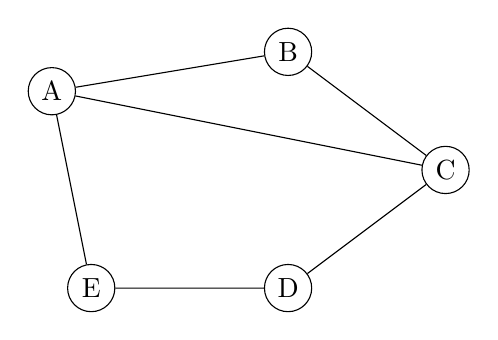
\begin{tikzpicture}[every node/.style={circle,draw,inner sep=1.5pt,minimum size=6mm}]
\node (a) at (0,2) {A};
\node (b) at (3,2.5) {B};
\node (c) at (5,1) {C};
\node (d) at (3,-0.5) {D};
\node (e) at (0.5,-0.5) {E};
\draw (a)--(b) (b)--(c) (c)--(d) (d)--(e) (e)--(a) (a)--(c);
\end{tikzpicture}
\end{center}

In this small graph, vertex A has degree 3, being joined to B, C, and E, while vertex E has degree 2. Every graph obeys the following law.

\begin{dingli}[Handshaking lemma]
In any graph, the sum of all vertex degrees is twice the number of edges.
\end{dingli}

\begin{proof}
Count edge by edge. Every edge has two endpoints and contributes 1 to the degree of each. The degree sum is therefore exactly twice the edge count.
\end{proof}

An immediate corollary is that \emph{every graph has an even number of odd-degree vertices}. The degree sum is even, and odd summands must occur in pairs to give an even sum. In party language, the number of guests who shake an odd number of hands is always even. Quietly check at your next party: this is a theorem, not a coincidence.

One especially clean class of graphs is \emph{trees}: connected graphs, with a path between every pair of vertices, containing no cycles. Like a real tree, a tree offers no route that loops back to its starting point. A basic fact is that a tree with $n$ vertices has exactly $n-1$ edges. Every edge is indispensable: deleting any one disconnects the graph. Family trees, computer folder hierarchies, and knockout-tournament brackets are trees. One important use is connecting everyone with as few edges as possible. Connecting 6 villages needs at least 5 roads; to minimise total construction cost, select the cheapest tree from the candidate edges. This is the minimum spanning tree problem, which admits simple, efficient greedy algorithms.

A more immediately practical problem is the \emph{shortest path}. Given a weighted graph with junctions as vertices, streets as edges, and lengths as weights, which route from home to school has minimum total length? You might suggest listing all routes and choosing the shortest, but as junctions multiply, the number of routes can explode like a factorial. In the 1950s, computer scientist Dijkstra devised a greedy algorithm: start at the origin, always process the vertex with the smallest currently known distance, and use it to update its neighbours' distance records. The search spreads out like ripples until reaching the destination. Each step makes only local comparisons, yet finds the globally shortest route, provided all edge lengths are nonnegative. Modern navigation software still uses enhanced versions of this central idea.

Replace lengths with capacities and we enter another world: \emph{network flow}. Imagine the graph as water pipes, each with a maximum flow rate determined by its size. What is the most water that can reach your house from the waterworks per unit time? Intuitively, bottlenecks limit the answer. Draw a line on the map separating the waterworks from your house; the total capacity of pipes crossing it bounds how much can pass through. The tightest of all such cuts determines the true limit. This is the celebrated \emph{max-flow min-cut theorem}: a network's maximum flow equals the capacity of its minimum cut. We will not prove it, but savour its form: a maximisation problem has exactly the same answer as a minimisation problem. Such ``maximum equals minimum'' duality recurs throughout mathematics, each time revealing a deep structural symmetry. Parcel sorting, power-grid scheduling, and even tournament scheduling all bear traces of network flow.

\section{Algorithms: Giving Machines a Route to Follow}

So far, we have solved problems with our own hands and minds. Real graphs, however, can have millions of vertices: a country's roads, or the links of the entire internet. We then need an \emph{algorithm}: a precise, mechanical list of steps that anyone, or any machine, can follow to obtain the answer. Algorithms are the meeting point of discrete mathematics and computer science.

There are two basic approaches to algorithm design, both already glimpsed in this chapter. The first is \emph{recursion}: break a problem into smaller problems of the same kind until they are small enough to answer directly. The stair-counting formula $f_n=f_{n-1}+f_{n-2}$ is recursive, as is traversing computer folders: ``list this folder's contents'' means ``repeat the listing procedure for every subfolder''. The second is \emph{search}: organise all possibilities into a decision tree and walk through it systematically. Solving a maze is a search: junctions are vertices, corridors are edges, and finding the exit means finding a path in this graph.

Search has two personalities. \emph{Depth-first search} is a single-minded explorer: follow one route to its end, then backtrack at a wall. \emph{Breadth-first search} spreads like ripples: first inspect everything reachable in one step, then in two. For shortest paths, this guarantees that the first exit found is nearest. Dijkstra's algorithm is essentially an upgraded breadth-first search for weighted graphs.

But ``able to compute an answer'' and ``able to afford the computation'' are different things. This calls for our final tool: an intuitive account of \emph{algorithmic complexity}.

\begin{shuyu}{Big O notation}
\textbf{Intuition}: Focus on how an algorithm's workload grows as the problem size $n$ increases, ignoring constant factors and minor details.

\textbf{Formal description}: If the workload is bounded by a fixed multiple of $n$, write $O(n)$; if bounded by a fixed multiple of $n^2$, write $O(n^2)$; and so on.

\textbf{Example}: Finding the largest of $n$ numbers takes $O(n)$ work, since each number need only be inspected once; listing all line-ups of $n$ people is $O(n!)$, hopelessly slow.
\end{shuyu}

Revisit the chapter through big O notation. Dijkstra's algorithm on a graph of $n$ vertices takes roughly $O(n^2)$ work: ten times as many junctions means about a hundred times as long, which is manageable. Checking every pairwise relationship among $n$ people is also $O(n^2)$, again manageable. But $O(2^n)$ or $O(n!)$ tells a different story: $2^{40}$ already exceeds a trillion, and $25!$ is astronomical. A problem size of only a few dozen can keep a machine running indefinitely. Famous hard problems include the travelling salesman problem: given cities, find the shortest tour visiting every city and returning to the start. Nobody yet knows whether a general algorithm can be fundamentally much faster than near-enumeration. This is one of computer science's greatest mysteries, usually written as the ``P versus NP problem'', with a million-dollar prize awaiting an answer.

Discrete mathematics therefore leaves us with a two-sided lesson. Graphs, recurrences, and greedy methods bring seemingly impossible large problems within computational reach. Complexity theory, meanwhile, marks the boundaries unsentimentally: some problems may be not merely beyond today's resources, but inherently intractable. Knowing which is which is itself deep mathematics.

\section{Discrete Structures, Cryptography, and Number Theory: Why They Belong Together}

This chapter appears to concern counting and connections, yet it stands alongside Chapter 13's number theory and the cryptography in your phone. There are three layers to the connection.

First, \emph{a computer is itself a discrete machine}. It stores strings of 0s and 1s and executes one instruction at a time, naturally inhabiting a discrete world. Even continuous quantities such as a circle's area must be broken into finite decimal representations inside a computer. The mathematics of discrete structures---combinatorics, graphs, logic, and recurrences---is therefore computer science's native language.

Second, \emph{cryptographic security comes from hard discrete problems}. Chapter 13 explained that multiplying two large primes is easy, while splitting their product back into primes is extremely difficult: this underpins RSA. Notice that the asymmetry is exactly a complexity issue: the forward operation is $O(\text{polynomial})$ multiplication, while the reverse currently has only slow, near-enumerative algorithms. Discrete logarithms and shortest vectors in lattices likewise underpin modern cryptography. At the other end, the pigeonhole principle watches over hash functions, which compress messages of arbitrary length into fixed-length fingerprints. Infinitely many messages and finitely many fingerprints guarantee collisions. Cryptographers must make \emph{finding} a collision computationally infeasible.

Third, \emph{number theory is itself discrete mathematics}. Integers come one at a time; primes are scattered points on the number line. Combinatorial tools continually serve number theory. Binomial coefficients conceal traces of primes: when $p$ is prime, $\binom{p}{1},\binom{p}{2},\dots,\binom{p}{p-1}$ are all divisible by $p$; try $p=5$ yourself. Divisibility in recurrent sequences is a staple of competitions and research, and graph theory even helps investigate distances between primes.

\begin{lianjie}
\textbf{Looking ahead}: The multiplication principle and factorials return in Chapter 18's probability: an equally likely sample space is really a combinatorial count. Graph connectivity and cycles are generalised through the Euler characteristic in Chapter 16's topology. Chapter 19 explores algorithms and the limits of computability further.

\textbf{Looking back}: Chapter 7's matrices can record a graph's connections in an adjacency matrix. Multiplying the matrix by itself counts two-step paths: linear algebra and graph theory shake hands here. Chapter 13's congruences and primes jointly underpin divisibility properties of binomial coefficients and cryptographic applications.
\end{lianjie}

\section{Mathematical Experiments}

\begin{shiyan}
\textbf{Experiment 1: Counting trees.} Draw 4 vertices and try to draw every non-isomorphic tree, meaning fundamentally different connection patterns. How many are there? Repeat with 5 vertices. (There are 2 with 4 vertices and 3 with 5.) Notice how quickly the sequence grows: with 10 vertices there are already 106.

\textbf{Experiment 2: Shortest paths by hand.} Draw a small graph with 5 junctions: home, school, park, bookshop, and station. Add seven or eight edges as you please, labelled with lengths. Following Dijkstra's idea, start at home and mark each junction with its currently known shortest distance. Each time you process a junction, update its neighbours. Compare your result with the route you guessed by eye.

\textbf{Experiment 3: Binomial coefficients and primes.} Calculate $\binom{5}{1},\binom{5}{2},\binom{5}{3},\binom{5}{4}$ and check whether all are divisible by 5. Repeat for $n=6$ and see whether the conclusion survives. What makes the difference?
\end{shiyan}

\begin{toolbox}
New tools for our collection:
\begin{itemize}
\item \textbf{Addition and multiplication principles}: Add across categories, multiply across steps; first ask whether anything is counted twice.
\item \textbf{Permutations and combinations}: For ordered choices use $A_n^k=\dfrac{n!}{(n-k)!}$; for unordered choices use $\dbinom{n}{k}=\dfrac{n!}{k!(n-k)!}$.
\item \textbf{Recurrences}: Define the current problem using smaller problems of the same kind, as in $f_n=f_{n-1}+f_{n-2}$.
\item \textbf{Binomial theorem}: The coefficients of $(a+b)^n$ are combination numbers; setting $a=b=1$ gives $2^n$ subsets.
\item \textbf{Pigeonhole principle}: More pigeons than holes force collisions, the prototype of unavoidable-collision arguments.
\item \textbf{Graph language}: Vertices, edges, and degrees; the handshaking lemma $\sum\text{degrees}=2\times\text{number of edges}$.
\item \textbf{Trees, shortest paths, network flow}: Connected, edge-efficient skeletons; greedy expansion; maximum flow equals minimum cut.
\item \textbf{Big O notation}: Use growth rates ($O(n)$, $O(n^2)$, $O(2^n)$, $O(n!)$) to judge whether an algorithm can finish.
\end{itemize}
\end{toolbox}

\begin{pandeng}
Directions for further climbing:
\begin{itemize}
\item \textbf{Generating functions}: Compress a sequence $a_0,a_1,a_2,\dots$ into a function and solve recurrences algebraically; the Fibonacci closed formula can be derived this way.
\item \textbf{Ramsey theory}: Three mutual acquaintances or strangers among six people is only the beginning. More generally, sufficiently large structures inevitably contain sufficiently orderly substructures: the mathematics of the impossibility of total disorder.
\item \textbf{P versus NP}: The gap between verifying and solving, one of the Clay Mathematics Institute's seven Millennium Prize Problems.
\item \textbf{Spectral graph theory}: Study connectivity through matrix eigenvalues, supporting search-engine page ranking.
\item \textbf{Extremal graph theory}: How many edges can a graph have under a restriction such as containing no triangles?
\end{itemize}
\end{pandeng}

\section*{Questions to Think About}

\textbf{Observation}
\begin{sikao}
\item Calculate $\binom{10}{2}$ and $\binom{10}{8}$: they are equal. Explain why $\binom{n}{k}=\binom{n}{n-k}$ always holds by comparing choosing 2 people to attend a meeting with choosing 8 to stay behind. \emph{Hint: every choice of $k$ objects simultaneously leaves $n-k$ objects behind.}
\item In your group or family, count how many other members each person knows. Add the degrees, check that the sum is even, and explain using the handshaking lemma. \emph{Hint: draw the acquaintance relationships as a graph.}
\end{sikao}

\textbf{Proof}
\begin{sikao}
\item Prove that a tree with $n$ vertices has exactly $n-1$ edges. \emph{Hint: induct on the number of vertices. A tree always has a leaf, a vertex of degree 1. Remove it and its incident edge to leave a smaller tree.}
\item Prove that among any 6 people, there are 3 pairwise acquaintances or 3 pairwise strangers. \emph{Hint: the text took us halfway. Fix one person and use the pigeonhole principle to find three sharing the same relationship with that person. Then distinguish whether any pair among the three has that same relationship.}
\end{sikao}

\textbf{Challenge}
\begin{sikao}
\item Place $n$ equally spaced points on a straight line and join every pair by a segment. At least how many distinct midpoints do all these segments have? \emph{Hint: draw and count for $n=3,4,5$. Put the points at coordinates $1,2,\dots,n$; a midpoint has coordinate $\dfrac{i+j}{2}$. Which values can this take?}
\item Among 8 identical-looking gold coins, 1 is a lighter counterfeit. What is the minimum number of weighings on a balance without weights that guarantees finding it? If the counterfeit might be either lighter or heavier, how many weighings are needed for 12 coins? \emph{Hint: each weighing has three outcomes: left heavier, right heavier, or balance. Thus $k$ weighings distinguish at most $3^k$ possibilities. View each weighing as a branch in a decision tree.}
\end{sikao}

\section*{The Door to the Next Chapter}

We have learnt to count discrete objects: people in line, handshakes, edges in graphs. One phenomenon kept recurring: local rules for discrete objects, such as the divisibility of $\binom{p}{k}$ by a prime $p$, are often controlled by primes behind the scenes. But zoom out and ask a global question: how densely do these discrete prime points cover the entire number line?

Specifically, there are 25 primes up to 100, 168 up to 1000, and 78498 up to a million. Is there a formula for these numbers? Primes grow sparser, but at a uniform rate? Curiously, the strongest tools for answering this purely discrete question come from the most continuous world: calculus, infinite series, and even functions on the complex plane. Mathematicians discovered that a continuous shadow seems to guide prime distribution with precision. Its secret is concentrated in an object called the Riemann $\zeta$ function, which also carries mathematics' most famous unsolved mystery.

Discrete and continuous: these two apparently diverging rivers meet in the next chapter.
